\lab{Deep Learning}{Intro to Deep Learning and PyTorch}
\objective{Deep Learning is a popular method for machine learning tasks that have large amounts of data, including image recognition, voice recognition, and natural language processing.
In this lab, we use PyTorch to write a convolution neural net to classify images.
We also look at one of the challenges of deep learning by performing an adversarial attack on our model.}


\newcommand{\lieq}[1]{{\text{\li{#1}}}}

\section*{Intro to Neural Networks}

%This paragraph doesn't really have any very important information
%\begin{comment}
%The brain is a biological neural network that is composed of neurons that are connected chemically and electrically.
%Signal are transferred from one neuron to another until they reach a target cell that acts on the signal.
%For instance, when you see a ball coming towards you, the signals travel along a certain path through the brain and trigger your arm to catch it. 
%Every movement of your body, both conscious and unconscious, is the result of signals traveling along these connections.
%These connections also play an important role in developing and losing memory, and are therefore instrumental in how a human learns.
%\end{comment}

An \emph{artificial neural network} is a machine learning tool inspired by the idea of neurons passing information between each other to learn.
The network is composed of layers of neurons, usually called \emph{nodes}, that are connected in various ways.
Each connection has a \emph{weight} based on its importance, which is used as information is passed through the network from one layer to the next.
For example, in Figure \ref{fig:neuralnet}, the yellow input is passed to the first layer, blue, then the green layer, and then to the final output layer.
%For example, if you were trying to catch a ball, the only thing that you're aware of is the input of the incoming ball, and the output of your hand being raised.
%Everything else happens unconsciously and is hidden from your perception.
%Similarly, the middle layers for a neural network are considered ``hidden'' because they're not directly viewable to the outside world.

The middle layers for a neural network are considered ``hidden'' because they're not directly viewable to the outside world. 
You can view them but they will be a mess of seemingly random numbers, not the helpful classification labels you would get from an end layer.


\begin{figure}[h]
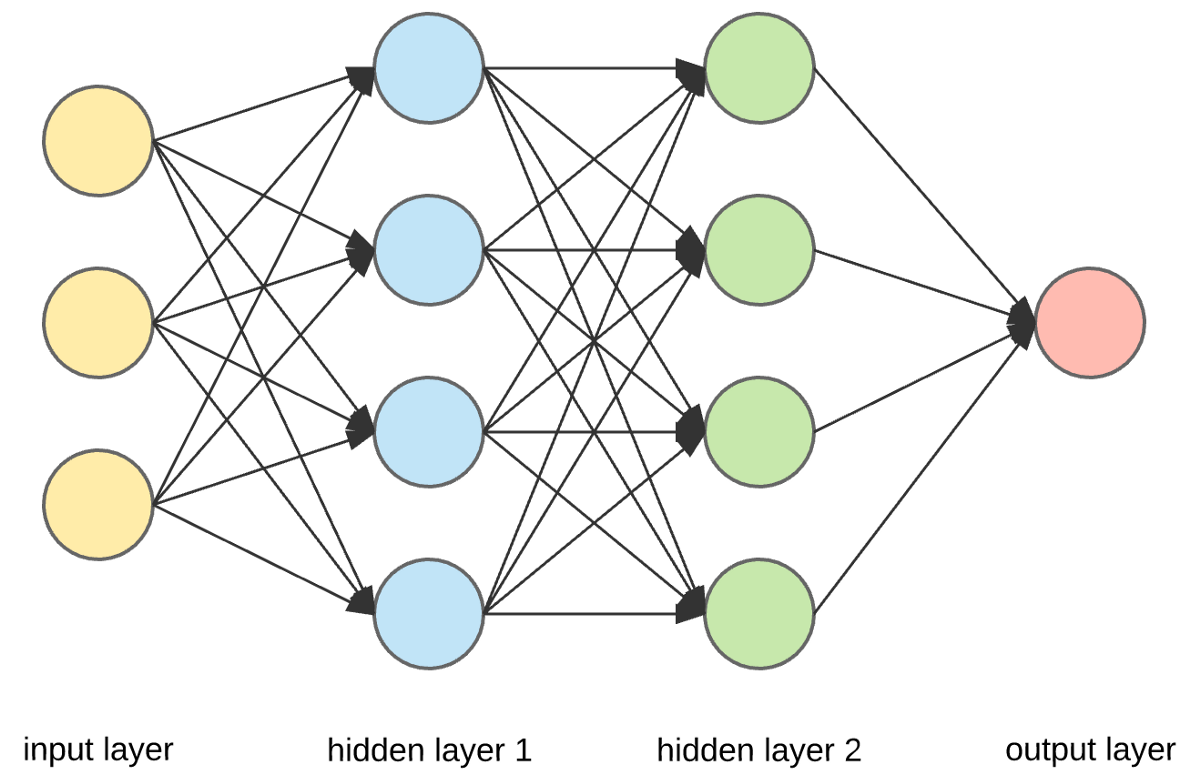
\includegraphics[width=10cm]{figures/neural_net.png}
\caption{A high level diagram of an artificial neural network.}
\label{fig:neuralnet}
\end{figure}

In a neural network, the input is often images, text, or sounds represented as a vector of real numbers.
%The input vector is first sent to the initial hidden layer and multiplied by the weights of their respective edges.%, to get a measure of importance.
%A vector called the \emph{bias} of the layer is added to offset these values in certain ways.
In order to evaluate a network, these values are then multiplied by the weight of each pertinent edge, and all respective values are added up to create the node value.
A vector called the \emph{bias} of the layer is added to each respective node, finalizing the linear combination step.
An \emph{activation function} takes these node values and applies a nonlinear transformation to them, which allows the model to learn complex nonlinear transformations between the input and output.
Without these activation functions, the network would be linear and exactly the same as a network with no hidden layers.
Mathematically, a typical neural network looks like the nested function composition
\[
f_N(\mathbf{x}) = \mathbf{a}(W_k\mathbf{a}(\ldots\mathbf{a}(W_2\mathbf{a}(W_1\mathbf{x}+\mathbf{b}_1)+\mathbf{b}_2)\ldots)+\mathbf{b}_k)
\]
where \(\mathbf{a}\) is the activation function, and \(W_i\) and \(\mathbf{b}_i\) are the weights and biases of each layer of the neural network.
The model is trained by adjusting the weights and biases, typically using a variant of gradient descent, until the model output accurately matches the training labels.


\section*{Intro to PyTorch}

PyTorch is an open source machine learning library developed by Facebook AI Research.
%It has two main capabilities: deep neural networks and GPU tensor computing.
%Deep neural networks are neural networks with many hidden layers.
It's mainly used for fast GPU processing of deep neural networks (neural networks with many hidden layers).
%Their training is possible through automatic differentiation, an algorithm that allows the calculation of derivatives automatically, accurately, and quickly.
%With the amount of data used in neural networks, GPUs significantly speed up the entire process.
GPUs (graphics processing units) are designed to compute thousands of operations at once and are vital for parallelizing the operations used by neural networks, which is why they are used here.
For more information and documentation on PyTorch, visit \url{https://pytorch.org/}


We will be working in Google's Colaboratory, \url{https://colab.research.google.com/notebooks/intro.ipynb}.
Colab notebooks use Google's cloud servers, which have a built-in GPU.
To enable the GPU in a Colab notebook, select the \textit{Runtime} tab and then \textit{Change runtime type}.
This will open a popup called \li{Notebook Settings}.
Under \textit{Hardware Settings}, select GPU.

We can verify that GPU is enabled by calling \li{torch.cuda.is_available()}.
If this function returns \li{False}, a GPU is not available, and the code will be run on the CPU.

\begin{comment}
\begin{warn}
Colab has a limit on the amount of GPUs available and the longer one runs a notebook, the less priority one has.
As we will use this feature for both this lab and the Recurrent Neural Networks lab, it is advisable to not leave the GPU active while you are not using it.
Note that enabling or disabling the GPU resets the notebook environment, so be sure that you save the results of any important computations before doing so.
%TODO test if it also removes files uploaded to the colab session. If it does might not be worth including this
%TODO I'm pretty sure it does, but it's really not that bad. Way less time consuming than a GPU timeout - Bryce
\end{warn}
\end{comment}

CUDA is a parallel computing platform %developed by Nvidia
 for GPU computing.
 The PyTorch package \li{torch.cuda} interfaces with this package and allows code to be run on the GPU.
 
PyTorch represents vectors and arrays using \emph{tensors}.
A tensor is a data structure similar to a numpy array that is designed to be compatible with GPUs.
Like a numpy array, it has a shape, data type, and can be multi-dimensional.

In order for a tensor to be used by the GPU, it must be stored on the GPU.
A tensor can be sent directly to the GPU using \li{variable.cuda()}; however, if the GPU is not available, this will cause an error.
A more flexible approach is store which deivce we are doing computations on as a variable \li{device}.
We will prefer to use a GPU if available, but will use the CPU if a GPU is not available.
Then, we can send our variables to the correct location in both cases by using \li{variable.to(device)}:

\begin{lstlisting}
>>> import torch

>>> x = torch.tensor([3., 4.])					# Create tensor on CPU
>>> y = torch.tensor([1., 2.]).cuda()			# Create tensor on GPU

# Create the device, choosing GPU if available
>>> device = torch.device("cuda:0" if torch.cuda.is_available() else "cpu")
>>> z = torch.tensor([1., 2.]).to(device)		# Create tensor on device
\end{lstlisting}
You can check which device a variable is on by displaying it.
If it is on a GPU, it will list which number it is.
\li{cuda:0} means that the device running is the default GPU.
If you are using a machine that has multiple GPUs, you can set the device to be a specific GPU by changing the number. 
In Colab, only \li{cuda:0} is available.
\begin{lstlisting}
>>> x
tensor([3., 4.])								# Check location of x (CPU)

>>> x = x.to(device)							# Move x to GPU
>>> x											# Check location of x (GPU 0)
tensor([3., 4.], device='cuda:0')							
\end{lstlisting}

\begin{warn}
Cross-GPU operations are not allowed.
This means that the model and data must all be on the same device.
If the model is called on data that is on a different device, say the model is located on the GPU and the data is on the CPU, you will get the following runtime exception:
\begin{lstlisting}
RuntimeError: Input type (torch.FloatTensor) and weight type (torch.cuda.FloatTensor) should be the same.
\end{lstlisting}
If you get this error, you will need to move one the variables so that they are all on the same device.
\end{warn}

\subsection*{Data}
For this lab, we will be using the CIFAR10 dataset.
It consists of $60,000$ images of size $32\times32$, represented as a $3\times 32\times 32$ matrix, where the 3 channels describe the colors using RGB.
The images are evenly split into ten classes represented by the numbers $0-9$:  airplanes, cars, birds, cats, deer, dogs, frogs, horses, ships, and trucks.

For convenience, the dataset is already split into a training and a testing set; however, we will also add a \emph{validation} set.

Using a train-validate-test split is good practice in general, because usually we will want to test and compare different models and hyperparameter choices iteratively until we arrive at one that works well for our problem.
Once we are done training, we would like to use the test set to determine how well our model fits the data.
However, if we use the test set to compare how well each of our models performs, it effectively becomes a second train set that we are learning by trying different models, and using the test set to determine how well our model works on the whole dataset is no longer really valid.
As such, it is better practice to use a three-way split.
We train each model on the train set, use the validation set to compare the models, and use the test set to determine if our final model appears to fit the data well.

The CIFAR10 dataset is split into a train set of 50,000 images and a test set of 10,000 images. We will split the original train set into a new train set of 40,000 images and a validation set of 10,000 images.
To use the data, we must transform it into PyTorch tensors.
%When using PyTorch, all of the data must be in tensor form so that it can be moved to a GPU.
We also will normalize the data, as this generally improves the results.
We will normalize the values to have mean 0 and standard deviation 1 for each component.
Finally, we will split the dataset and place it inside a \li{torch.utils.data.DataLoader} class for easier manipulation.

To load the dataset, we use the \li{torchvision.datasets.CIFAR10} function, which accepts a folder for the data to be stored in.
Some important keyword arguments are listed in Table \ref{table:deeplearning:download_data}.
\begin{table}[H]
	\centering
	\begin{tabular}{c|p{0.5\linewidth}}
	Parameter & Explanation \\
	\hline
	\li{train} & Whether to get the training data or the test data.\\
	\li{download} & Whether to download the data.
	You usually only need this the first time you access the dataset.
	Note that restarting Google Colab will require re-downloading the data, however.\\
	\li{transform} & Applies the given \li{transform} when loading the data.
	This transform always should convert the data into a PyTorch tensor.
	\end{tabular}
	\caption{Parameters of the \li{datasets.CIFAR10} loading function}\label{table:deeplearning:download_data}
\end{table}
We can use the \li{transform} parameter in particular to easily normalize our data.
PyTorch has a module \li{torchvision.transforms} to make creating these transformations easier.
In this case, we want to use \li{transforms.ToTensor} to convert the data into tensors, and then \li{transforms.Normalize} to normalize the data.
The \li{Normalize} object accepts the desired mean and standard deviation after normalization.
We can use \li{transforms.Compose} to combine these together into a single transform object:
\begin{lstlisting}
>>> from torchvision import transforms

# Transform data into a tensor and normalize
>>> transform = transforms.Compose([
...        transforms.ToTensor(),
...        transforms.Normalize((0.0, 0.0, 0.0), (1.0, 1.0, 1.0))
...])
\end{lstlisting}
We can then load the data:
\begin{lstlisting}
>>> from torchvision import datasets

# Download the CIFAR10 training data to ../data
>>> train_data = datasets.CIFAR10('../data', train=True, download=True, transform=transform)
\end{lstlisting}
The data can then be accessed using indexing. 
Each data point is a tuple consisting of the $3\times32\times32$ image and its class.
You can also see the specs of the dataset by calling it without an index.

\begin{lstlisting}           
# Get the first training data point
>>> train_data[0]
(tensor([[[ 0.2314, ..., 0.5804],
          [ 0.0627, ..., 0.4784],
          ...,
          [ 0.7059, ..., 0.3255],
          [ 0.6941, ..., 0.4824]],
 
         [[ 0.2431, ..., 0.4863],
          [ 0.0784, ..., 0.3412],
          ...,
          [ 0.5451, ..., 0.2078],
          [ 0.5647, ..., 0.3608]],
 
         [[ 0.2471, ..., 0.4039],
          [ 0.0784, ..., 0.2235],
          ...,
          [ 0.3765, ..., 0.1333],
          [ 0.4549, ..., 0.2824]]]), 6)

# Get the class of the first training data point
>>> train_data[0][1]
6

# Get the specs of the CIFAR10 training set
>>> train_data
Dataset CIFAR10
    Number of datapoints: 50000
    Root location: ../data
    Split: Train
    StandardTransform
Transform: Compose(
               ToTensor()
               Normalize(mean=(0.0, 0.0, 0.0), std=(1.0, 1.0, 1.0))
           )
\end{lstlisting}

\begin{problem}
Create the \li{device} variable as indicated above.
Download the CIFAR10 training and test datasets, transform them into tensors, and normalize them as described above.
\end{problem}

PyTorch has a special class \li{DataLoader} that splits the data into batches for easy manipulation.
Sending individual data points to the GPU one at a time to be processed by our model is very inefficient, as it makes it impossible for the GPU to parallelize the computations.
Instead, we use \emph{batches}, and send multiple data points together.
Using larger batch sizes allows us to take advantage of GPUs, speeding up the training time.
Storing all of the data on the GPU is, however, generally impossible due to memory constraints.
Using too large of a batch size will cause out of memory issues, and tends to reduce the effectiveness of training.
Typical batch sizes are powers of $2$: 32, 64, 128, 256.

The \li{DataLoader} class accepts the dataset as its first argument.
The dataset can be a dataset object like the one we created above, a list containing the data points, or any iterable.
For the train set, we will first split the loaded data into two lists to create the actual train and validation sets.
The dataset object does \emph{not} support fancy indexing, so this step should be done with list comprehension:
\begin{lstlisting}
>>> actual_train_data = [train_data[i] for i in range(40_000)]

>>> from torch.utils.data import DataLoader

# Create a DataLoader from the shuffled training data
>>> train_loader = DataLoader(actual_train_data, batch_size=36, shuffle=True)
# and similarly for the validation set
\end{lstlisting}
The data is not ordered by its classes, so directly indexing like this will put a good mixture of all of the classes into both sets.
For the test set, we can just directly pass the dataset object into the \li{DataLoader}.
Some other useful parameters of the \li{DataLoader} class are listed in Table \ref{tabel:deeplearning:DataLoader}.

\begin{table}[h]
	\centering
	\begin{tabular}{c|p{0.5\linewidth}}
		Parameter & Explanation \\
	\hline
		\li{batch_size} & The size of batch to use \\
		\li{shuffle} & Whether to shuffle the data \\
		\li{num_worker} & The number of processes to use, in order to load the data in parallel \\
	\end{tabular}
	\caption{Parameters of the \li{DataLoader} object}\label{tabel:deeplearning:DataLoader}
\end{table}

Once we have the data in the \li{DataLoader} class, we can iterate through it to get data points.
We can turn it into an iterator using the \li{iter} method, and then get batches one-at-a-time using the \li{next} method:
\begin{lstlisting}
# Get the 36 images of size 3x32x32 and labels in the first batch
>>> dataiter = iter(train_loader)   
>>> images, labels = next(dataiter)
>>> images.size()
torch.Size([36, 3, 32, 32])

>>> images[0].size()
torch.Size([3, 32, 32]) 

>>> labels[0]
tensor(8)
\end{lstlisting}
This method is particularly useful if we just need a few images.
We can also directly iterate through all of the images using a \li{for} loop:
\begin{lstlisting}
>>> for batch, (x, y_truth) in enumerate(train_loader):
...    # Move to the GPU
...    x, y_truth = x.to(device), y_truth.to(device)
...    # ...
\end{lstlisting}
This will be a more convenient method for training.

\begin{problem}
Split the data into train, validate, and test sets, and create DataLoaders for each one. 
The train set should have 40,000 data points and the test and validate sets should each have 10,000 data points. 
Use a batch size of 32 for the training set and 1 for the validation and test sets.
Specify \li{shuffle=True} for the training set, and \li{shuffle=False} for the validation and test sets (this is common practice in deep learning).
\end{problem}

\section*{Neural Networks in PyTorch}
Before creating a good model for this dataset, we will start with a simple model to illustrate how to set up a neural network in PyTorch.
This model will use only fully-connected linear layers and activation functions.
First, we need to import the \li{nn} module, which contains all of the classes we need for this:
\begin{lstlisting}
from torch import nn
\end{lstlisting}

\subsection*{Simple layers}
A linear layer takes an input vector \(x\) and outputs \(Ax+b\) for a learned weight matrix \(A\) and bias vector \(b\).
This is implemented in Pytorch as \li{nn.Linear(in_features, out_features)}, where \li{in_features} is the length of the input vector and \li{out_features} is the desired length of the output vector.
This is called a \emph{fully-connected} layer, because every entry of \(A\) and \(b\) are allowed to be nonzero.

After each layer, we want to pass the values through an \emph{activation function}.
This allows the model to be nonlinear, allowing it to learn much more complicated behaviors than it would otherwise.
The most commonly used activation function is the Rectified Linear Unit (ReLU) function:
\[
\mathrm{ReLu}(x) = \max(0,x)=\begin{cases}
x  & x>0
\\
0 &\text{otherwise}
\end{cases}
\]
This activation function avoids many issues that other activation functions have, and is used almost universally.
For the final activation function, however, we will use a different activation function: the \emph{softmax} function
\[
\mathrm{Softmax}(x_1,\ldots,x_n)=\left(\frac{e^{x_1}}{\sum_{i=1}^n e^{x_i}},\ldots,\frac{e^{x_n}}{\sum_{i=1}^n e^{x_i}}\right).
\]
The components of the output of the softmax function are all non-negative and sum to 1.
This allows the output of the final layer to be interpreted as probabilities, which is useful for classification.
The component with the highest probability will be the neural network's prediction for the input image.
This also enables the use of cross-entropy as a very natural loss function, which will be discussed later.
These two activation functions are available as \li{nn.ReLU} and \li{nn.Softmax}.

\begin{warn}
    The cross-entropy loss function from PyTorch, \li{nn.CrossEntropyLoss}, combines logarithmic softmax \li{log_softmax} and the negative log likelihood loss \li{NLLLoss}, 
    which means you should NOT apply softmax as the last layer of your model.
    
    Performing softmax twice can cause numerical instabiility in the model's accuracy.
\end{warn}

\subsection*{Creating a model}
To create a neural network in PyTorch, we begin by creating a class that inherits from \li{nn.Module}:
\begin{lstlisting}
class NNExample(nn.Module):
\end{lstlisting}
The class \li{nn.Module} handles internals so that training is simpler, as well as providing a variety of useful methods.
In the initializer of our class, we need to call the \emph{superconstructor} \li{super().__init__()} to initialize the \li{nn.Module} itself.
Then, we initialize all of the layers we want to use in our model.
For this example, we will use two fully-connected linear layers with activation functions after each.
Since our inputs are \(3\times32\times32\) tensors and linear layers only work with vectors, we will also include an \li{nn.Flatten} layer.
\begin{lstlisting}
    def __init__(self):
        # Initialize nn.Module
        super().__init__()
        
        # Create our layers
        self.flatten = nn.Flatten()
        self.linear1 = nn.Linear(in_features=3*32*32, out_features=100)
        self.relu = nn.ReLU()
        self.linear2 = nn.Linear(in_features=100, out_features=10)
\end{lstlisting}
We need to set all of these layers as members of our class in order for them to be properly detected in the training process.
Notice that the input dimension of the first layer (\li{linear1}) is equal to the dimension of the (flattened) input image ($3\times32\times32$), but from there, the output dimension is chosen arbitrarily to be 100.
The second layer (\li{linear2}) must then have input dimension equal to the output dimension of \li{linear1}, but its output dimension is chosen to be 10, which is the number of classes possible in the CIFAR10 dataset.

Lastly, we define the \li{forward()} method, which calls all of the layers on an input image to give us the output:
\begin{lstlisting}
    def forward(self, x):
        x_flat = self.flatten(x)
        x_layer1 = self.relu(self.linear1(x_flat))
        output = x_layer1
        return output
\end{lstlisting}
Even though each layer is really a class (note how we initialize them in \li{__init__()}), we can call them as if they are functions.
Any layer that contains \emph{learnable parameters} (for example, the weights present in linear layers), must be called individually in the \li{forward()} method, as otherwise this would force it to reuse the parameters and reduce training effectiveness.
However, for layers that do not have learnable parameters, such as activation functions, we can safely reuse them and call them multiple times in the \li{forward()} method.
Hence, \li{nn.ReLU()} only needs to be defined once in the \li{__init__()} method, even when it may be called multiple times in the \li{forward()} method.

This neural network would likely perform very poorly on the CIFAR10 dataset, however; only using fully-connected linear layers does not work well for images.
For a better method, we will turn to \emph{convolutional neural networks}.

Convolutional neural networks (CNNs) are a type of neural network that use \emph{convolution layers}.
They also commonly use \emph{pooling layers}
They are particularly well-suited to working with images, such as the CIFAR10 dataset.
We now discuss these components and how to use them in PyTorch.

\subsection*{Convolution Layers}
A convolution layer takes a two-dimensional array of weights called a \emph{kernel} (sometimes called a filter) and multiplies it by the input at all possible locations, ``sliding'' around the input.
It is particularly useful when working with images, as it preserves and extracts spacial structures, unlike fully-connected linear layers.

Consider the following $5\times 5$ input image and $3\times 3$ kernel:
\begin{table}[H]
\parbox{.45\linewidth}{
\centering
\begin{tabular}{|c|c|c|c|c|}
\hline
2 & 4 & 7 & 6 & 2\\
\hline
9 & 7 & 1 & 2 & 1\\
\hline
8 & 3 & 4 & 5 & 8\\
\hline
4 & 3 & 3 & 1 & 2\\
\hline
5 & 2 & 1 & 5 & 3\\
\hline
\end{tabular}
\label{tab:input}
\caption*{5$\times$5 Input Image}
}
\hfill
\parbox{.45\linewidth}{
\centering
\begin{tabular}{|c|c|c|}
\hline
1 & 0 & -1\\
\hline
1 & 0 & -1\\
\hline
1 & 0 & -1\\
\hline
\end{tabular}
\label{tab:input}
\caption*{3$\times$3 Kernel}
}
\end{table}

\noindent
To get each value in the output, the kernel is multiplied element-wise by $3x3$ squares inside the input and summed.
For the top left square in this example, the output is 
\[
2\cdot 1 + 4\cdot 0 + 7\cdot (-1) + 9\cdot 1 + 7\cdot 0 + 1\cdot (-1) + 8\cdot 1 + 3\cdot 0 + 4\cdot (-1) = 7.
\]
\begin{table}[H]
\parbox{.45\linewidth}{
\centering
\begin{tabular}{|c|c|c|c|c|}
\hline
$2\cdot 1$ & $4\cdot 0$ & $7\cdot (-1)$ & $6$ & 2\\
\hline
$9\cdot 1$ & $7\cdot0$ & $1\cdot (-1)$ & 2 & 1\\
\hline
$8\cdot 1$ & $3\cdot0$ & $4\cdot (-1)$ & 5 & 8\\
\hline
4 & 3 & 3 & 1 & 2\\
\hline
5 & 2 & 1 & 5 & 3\\
\hline
\end{tabular}
\label{tab:input}
\caption*{5$\times$5 Input Images}
}
\hfill
\parbox{.45\linewidth}{
\centering
\begin{tabular}{|c|c|c|}
\hline
7 & \(\cdots\) & \\
\hline
\(\vdots\) &  & \\
\hline
 & & \\
\hline
\end{tabular}
\label{tab:input}
\caption*{3$\times $3 Output}
}
\end{table}
\noindent
The $7$ represents a feature of the $3\times 3$ block in the top left corner. 
With a trained network applied to the image, these features can represent things such lines, curves, and colors, or even more complicated objects like a nose.

The \emph{stride} of a convolution is how much the kernel slides at a time as it passes over the input.
With out example, if the kernel slides one spot over (has a stride of 1), there will be $9$ submatrices inside the input image that will be used, and we would get a \(3\times 3\) matrix as output.
If we used a stride of 2 instead, only the top-left, top-right, bottom-left, and bottom-right submatrices would be used.

Notice that as the kernel slides around the image, the inside values are used in more multiplications than the outside value, causing us to lose information, especially about the corners.
If we want to keep more infomation about the edges of the image, we can use \emph{padding}.
Padding consists of adding a border around the input, usually filled with zeros.
This can also allow the output of the layer to be the same size as the input.
\begin{table}[H]
\parbox{.45\linewidth}{
\centering
\begin{tabular}{|c|c|c|c|c|}
\hline
2 & 4 & 7 & 6 & 2\\
\hline
9 & 7 & 1 & 2 & 1\\
\hline
8 & 3 & 4 & 5 & 8\\
\hline
4 & 3 & 3 & 1 & 2\\
\hline
5 & 2 & 1 & 5 & 3\\
\hline
\end{tabular}
\caption*{5$\times$5 input image}
}
\hfill
\parbox{.45\linewidth}{
\centering
\begin{tabular}{|c|c|c|c|c|c|c|}
\hline
0 & 0 & 0 & 0 & 0 & 0 & 0\\
\hline
0 & 2 & 4 & 7 & 6 & 2 & 0\\
\hline
0 & 9 & 7 & 1 & 2 & 1 & 0\\
\hline
0 & 8 & 3 & 4 & 5 & 8 & 0\\
\hline
0 & 4 & 3 & 3 & 1 & 2 & 0\\
\hline
0 & 5 & 2 & 1 & 5 & 3 & 0\\
\hline
0 & 0 & 0 & 0 & 0 & 0 & 0\\
\hline
\end{tabular}
\caption*{5$\times$5 input image padded with 0}
}
\end{table}


Each dimension of the output for a convolution layer is calculated as follows:
\[
\frac{\text{input size} - \text{kernel size} + 2\cdot \text{padding size}}{\text{stride}} + 1
\]
In our example with stride 1, kernel size 3, and no padding, the output size is $(5-3+2\cdot0)/1+1 = 3$.
It is good to ensure that the stride always divides the numerator, as otherwise the kernel will be applied asymetrically to the image.
Calculating the output dimension of a layer is necessary since the following layer will have its \emph{input} dimension size equal to the previous \emph{output} dimension size.

% this one is probably a confusing explanation, but at least it explains it now
One last feature that we need to discuss is \emph{channels}.
Image data (including ours) typically has three channels, representing the red, green, and blue contents of pixels.
Channels act like different ``layers'' of the image or of the convolutional output.
In a convolutional layer, there is one kernel for each pair of input channel and output channel.
If we have \(n\) input and \(m\) output channels, then we will have \(mn\) total kernels that are learned individually.
Each kernel is applied to its corresponding input channel as described above.
Then, each output channel is determined as the sum of the results of the convolutions of all of its kernels, plus a learned bias value.

Convolutional layers are represented in PyTorch with \li{nn.Conv2d}.
The constructor of this class requires three parameters \li{in_channels}, \li{out_channels}, and \li{kernel_size}.
It also has optional arguments \li{stride} (default 1) and \li{padding} (default 0).
Note that for each of the kernel size, stride, and padding, only an integer needs to be specified, and it will be used for both the x and y directions.
The following creates a convolutional layer that accepts an image with 3 channels, output 8 channels, and uses a \(3\times 3\) kernel with stride 1 and no padding:
\begin{lstlisting}
layer = nn.Conv2d(in_channels=3, out_channels=8, kernel_size=3)
\end{lstlisting}


\subsection*{Pooling layers}

Pooling layers are used to reduce the size of the image while retaining important information.
The input image is broken into small pieces, called \emph{pools}, each of which is condensed to a single number.
The most common form of pooling is \emph{max pooling}, where the output of each pool is just the maximum of its inputs.

\begin{table}[H]
\parbox{.45\linewidth}{
\centering
\begin{tabular}{|c|c||c|c|}
\hline
4 & 7 & 6 & 2\\
\hline
7 & 1 & 2 & 1\\
\hline
\hline
3 & 3 & 1 & 2\\
\hline
2 & 1 & 5 & 3\\
\hline
\end{tabular}
\label{tab:input}
\caption*{4$\times$4 Input Image}
}
\hfill
\parbox{.45\linewidth}{
\centering
\begin{tabular}{|c|c|}
\hline
7 & 6\\
\hline
3 & 5\\
\hline
\end{tabular}
\label{tab:input}
\caption*{2$\times$2 output after max pooling}
}
\end{table}
Max pooling has the particularly nice property of making the output remain similar if the input image is shifted slightly.

Max pooling layers are represented in PyTorch as \li{nn.MaxPool2d}.
They accept a single parameter \li{kernel_size}; this is the size of each of the pools.
Using \(2\times2\) pools is the most common.
The following creates a pooling layer that uses a \(2\times 2\) pool size:
\begin{lstlisting}
layer = nn.MaxPool2d(kernel_size=2)
\end{lstlisting}

\subsection*{Parameters}

When working with neural networks, it can be useful to know how many learnable parameters our model has.
This particularly dictates the amount of space needed to store the model.
The number of parameters in each layer depends on the type of layer and its input and output sizes.
Table \ref{table:param_cts} lists how to calculate this number for the layer types we have discussed.

\begin{table}
	\centering
	\begin{tabular}{r|c}
	Layer type & Number of Parameters \\
	\hline
	Linear & \((\lieq{in_features}+1)*\lieq{out_features}\) \\
	Convolutional & \(\left(\lieq{in_channels}\cdot \lieq{kernel_size}^2 + 1\right)*\lieq{out_channels}\) \\
	Pooling & No parameters \\
	Flatten & No parameters \\
	Activation functions & No parameters \\
	\end{tabular}
	\caption{Parameter counts for layer types we use in this lab}
	\label{table:param_cts}
\end{table}

For example, the example neural network above would have
\begin{align*}
\text{(first linear layer)}\quad\quad&
(3\cdot32\cdot 32+1)\cdot100 
\\
\text{(second linear layer)}\quad&
+(100+1)\cdot10 = 308310 \text{ parameters,}
\end{align*}
and the example convolutional layer would have
\[
(3\cdot 3^2+1)\cdot 8 = 224 \text{ parameters.}
\]

\begin{problem}
Create a class for a convolutional neural network that accepts images as \(3\times32\times32\) tensors and returns 1D tensors of length 10, representing its predicted probabilities of each class.
Include at least the following:
\begin{itemize}
	\item Three convolutional layers, each followed by an activation function
	\item A max pooling layer
	\item Two linear layers
\end{itemize}
Choose the size of the layers so that your model has at least 50,000 parameters (use Table \ref{table:param_cts}), and print out this calculation in the Jupyter notebook file.
In practice, specifications of model architecture (i.e. number of layers, layer sizes, etc.) are chosen quite arbitrarily until something works.
As such, you may customize your model architecture to your liking, provided your model meets the requirements specified above.
%(Avoid having too many more parameters, however, as it may negatively impact training speed and quality)

Hint: It can be very helpful to keep track of the size of the image after each step, so you know what the input size should be for the next step.
The max pooling layer should occur immediately after a convolutional layer is passed through an activation function.
Additionally, you will need a \li{nn.Flatten} layer after the convolutional layers and before the linear layers.
You can check that your model works correctly by passing an (unsqueezed) image through it as demonstrated in the following code:

\begin{lstlisting}
>>> model = NNExample()
>>> model(images[0].unsqueeze(0))
tensor([[0.0952, 0.1120, 0.1019, 0.0992, 0.0955, 0.0984, 0.0886, 0.1326, 0.0966, 0.0800]], grad_fn=<AddmmBackward0>)
\end{lstlisting}
Note that your neural network will predict different probabilities for each of the categories.

\end{problem}

\subsection*{Training the Model}
Now that we have data and a model all set up, we need to train the model on the data.
We do this by iterating through the DataLoader, calling the model on the data, determining how well the model classified the data, and then optimizing the model weights.
We use a loss function, called the \emph{objective}, to calculate the loss, which is the difference between the model's predicted labels and the actual labels of the data.
A common classification loss function is Cross Entropy Loss
\begin{equation*}
    L_{CE} = -\sum_i a_i log(p_i),
    \label{eq:cel}
\end{equation*}
where $i$ represents each data point, $p_i$ is the softmax probability for each data point, and $a_i$ is the label for each data point.
PyTorch's \li{nn.CrossEntropyLoss()} conveniently handles all of this.

Once the loss is calculated by the objective, we can use it to optimize the model weights to make the loss smaller.
This can be done through \emph{backpropagation}, which calculates the partial derivatives of the loss function with respect to each weight, and then uses gradient descent to update every weight.
PyTorch has several predefined methods for optimization, but we'll use the popular \li{Adam} algorithm.
PyTorch accumulates gradients when backpropagating, which is sometimes desireable, but in our case it would cause the loss to increase.
To prevent this, we need to zero out the gradients before we perform each backpropagation. 
PyTorch streamlines this entire training sequence in a very clean way, as shown in the following:

\begin{lstlisting}
>>> import torch.optim as optim

# Define the objective and optimizer
>>> objective = nn.CrossEntropyLoss()
>>> optimizer = optim.Adam(model.parameters(), lr=1e-4)


# For each iteration of the DataLoader, do the following
>>> optimizer.zero_grad()             # Zero out the gradients
>>> y_hat = model(x)                  # Predict labels
>>> loss = objective(y_hat, y_truth)  # Calculate loss
>>> loss.backward()                   # Backpropagate to compute gradients
>>> optimizer.step()                  # Optimize and update the weights
\end{lstlisting}

An \emph{epoch} is a complete training sequence that trains over the entire DataLoader.
To improve the model's accuracy, we can train over many epochs.
A good guideline is to train the model for the number of epochs it takes for the loss to stop decreasing. 

The loss is calculated using the training data, but at the end of each epoch we also want to know how well the model performs with the validation data.
Before we determine the validation accuracy, we need to switch our model to evaluation mode so it doesn't continue training.
This is done by the simple command \li{model.eval()}, but it's important to switch the model back to training mode at the start of each epoch using \li{model.train()}
The validation accuracy is determined by simply iterating through the validation DataLoader, and seeing if the model can correctly predict each data point.
The validation accuracy is then computed by dividing the number of correct predictions by the total number of data points in the validation DataLoader.
\begin{lstlisting}
>>> model.eval()                        # switch to evaluation mode
>>> validation_score = 0
>>> for x, y_truth in validation_loader:
>>>     x, y_truth = x.to(device), y_truth.to(device)
>>>     y_hat = model(x)
>>>     if y_truth == y_hat.argmax(1):  # compare with greatest probability
>>>         validation_score += 1
>>> validation_accuracy = validation_score / len(validation_loader)
\end{lstlisting}
The validation accuracy does not determine the model's final accuracy.
The final accuracy is computed in the same way as the validation accuracy, but this time using the testing data, and it's only computed one time, when the model finishes training entirely.

TQDM is a python package that displays the progress of a for-loop, which can help estimate the remaining time.
TQDM is initialized outside the loop, then updated inside the loop, as follows:

\begin{lstlisting}
>>> from tqdm import tqdm

>>> loop = tqdm(total=len(train_loader), position=0)

>>> for epoch in range(num_epochs):
>>>     loop.set_description('epoch:{}, loss:{:.4f}'.format(epoch,loss.item()))
>>>		loop.update()

>>> loop.close()

epoch:1 loss:1.8585: : 1402it [00:17, 79.69it/s]
\end{lstlisting}

\begin{problem}
Send your model to the device and instantiate the objective and optimizer.
Train your model with a TQDM display, and calculate the Validation Accuracy after each epoch. 
Begin by initializing your TQDM loop, then for each epoch, do the following:

\begin{enumerate}
\item Set your model to training mode (\li{model.train()})
\item Instantiate an empty \li{loss_list}
\item For each batch in \li{train_loader}:
\begin{enumerate}
    \item Send \li{x} and \li{y_truth} to device
    \item Zero out the gradients 
    \item Use model to predict labels of \li{x}
    \item Calculate loss between predicted labels and \li{y_truth}
    \item Append loss (\li{loss.item()}) to \li{loss_list} (the \li{.item()} feature extracts the element from a tensor with only one element)
    \item Update TQDM loop 
    \item Backpropagate to compute gradients 
    \item Optimize and update the weights
\end{enumerate}
\item Save the loss mean as the mean of the losses in \li{loss_list}
\item Set your model to evaluation mode (\li{model.eval()})
\item Calculate and save validation accuracy
\end{enumerate}
Finish the training by closing your TQDM loop.
Train for 10 epochs, saving the mean loss and validation accuracy for each epoch.
Plot the mean losses and validation accuracies, which should resemble Figure \ref{fig:results}.
Lastly, print the final test score using the testing data, as described above.

\label{prob:train}
\end{problem}

\begin{figure}[H]
    \centering
    \begin{tabular}{cc}
    \includegraphics[width=.45\textwidth]{figures/training_updated.pdf} &
    \includegraphics[width=.45\textwidth]{figures/validation_updated.pdf}
    \end{tabular}
    \caption{Training Loss and Validation Accuracy for a CNN on CIFAR10.}
    \label{fig:results}
\end{figure}


\section*{Adversarial Attacks}
 
Just like any algorithm or software, deep learning is susceptible to attacks.
For deep learning models, this vulnerability most often manifests in the model being extremely sensitive to certain types of changes in the input that really should not matter.
This results in the model giving nonsensical results, which, while amusing, can cause major problems.
Examples of adversarial attacks against neural networks range from adding a small amount of noise to a picture of a panda, resulting in the model classifying the image as a gibbon with 99\% confidence \cite{goodfellow2015advesarial} to fooling facial recognition by printing a pair of eyeglasses \cite{goodfellow2017physical}.
When designing machine learning models, it is important to be aware of these issues so that their impact can be mitigated.

\begin{figure}[H] % Three graphs.
\centering

 	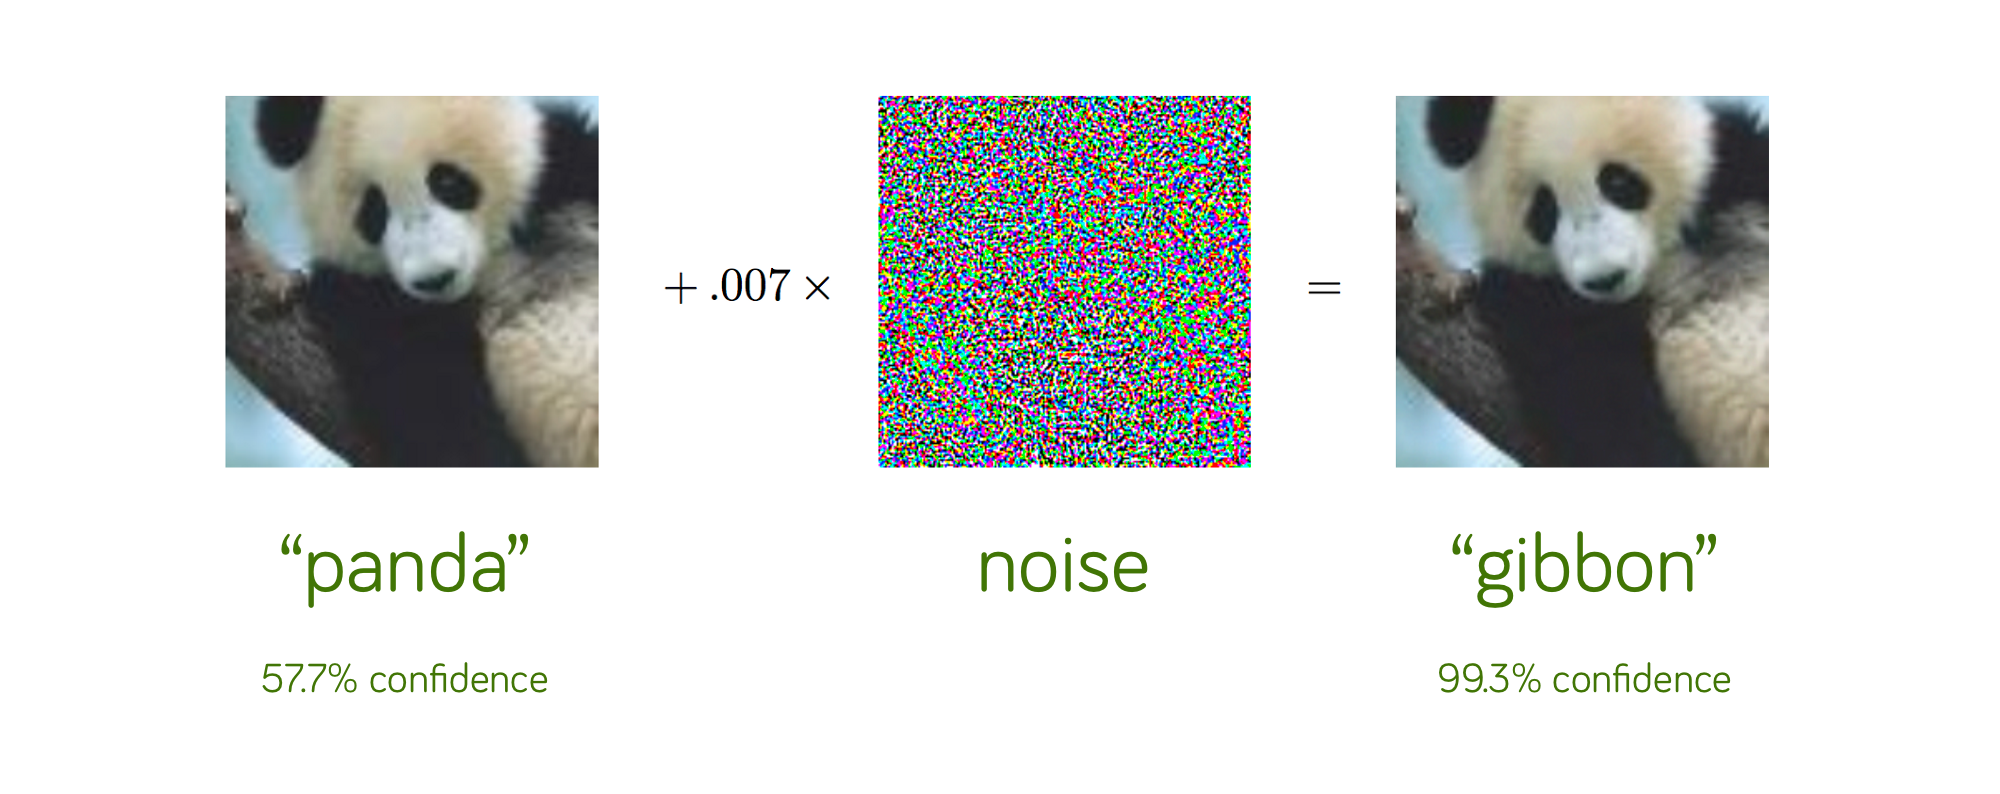
\includegraphics[width=\textwidth]{figures/panda.png}   
    \caption{A slight modification to a correctly-classified image of a panda results in the model confidently classifying it as a gibbon, despite the image not having changed in any substantial way.}
\end{figure}

The example of modifying the image of a panda is an attack called the \emph{Fast Gradient Sign Method (FGSM)}. 
FGSM is a \emph{white-box attack}, meaning that the attacker has access to the model; this is in contrast with a \emph{black-box attack} where the attacker only has access to the model's inputs and outputs.

During model training, gradients are used to adjust the model weights so that loss is minimized.
In FGSM, the gradient is instead used to perturb the input image in a direction that \emph{maximizes} the loss, using the following equation:
\begin{equation*}
x_\text{perturbed} = x + \epsilon\, \mathrm{Sign}(\nabla_x \mathrm{Loss}(\theta, x, y))
\end{equation*}
where $x$ is the input, $y$ is the label, and $\theta$ is the model parameters.


We can calculate this perturbation in PyTorch as follows.
To calculate the gradient of the model with respect to a piece of data \li{x}, we first need to set \li{x.requires_grad = True} and call \li{x.retain_grad()}. %the second part might not actually be necessary; further testing needed
Then, we zero out the optimizer's gradient, run \li{x} through the model, and compute the loss, similar to training.
After this, the gradient of the output with respect to \li{x} can be obtained using the attribute \li{x.grad.data}.

The following function \li{fgsm_attack} accepts a model and an image and performs the FGSM attack, returning the perturbed image:
\newpage
\begin{lstlisting}[belowskip=-0.8 \baselineskip]
def fgsm_attack(model, optimizer, objective, x, y, eps):
    """
    Performs the FGSM attack on the given model and data point x with label y.
    Returns the perturbed data point.
    """
    # Calculate the gradient
    x.requires_grad = True
    x.retain_grad()
    optimizer.zero_grad()
    output = model(x)
    loss = objective(output, y)
    loss.backward()
    data_grad = x.grad.data
    # Perturb the images
    x_perturbed = x + eps * data_grad.sign()
    
    return x_perturbed
\end{lstlisting}
We will use this function to explore this type of adversarial attack on our neural network.
\begin{comment}
\begin{algorithm}
\begin{algorithmic}[1]
\Procedure{Advesarial Attack}{model, data loader, $\epsilon$}
	\For{\pseudoli{x,y in test_loader}}		\Comment{Loop through test data}
		\State \pseudoli{x.requires_grad} $\gets$ \pseudoli{True}
		\State \pseudoli{output} $\gets$ \pseudoli{model(x)}
		\If{\pseudoli{output} $!= y$}		\Comment{Only modify correct images}
			\State \pseudoli{continue} 
		\EndIf
		\State \pseudoli{Update loss}
		\State \pseudoli{Zero out gradients}
		\State \pseudoli{Backwards step}
		\State \pseudoli{data_grad} $\gets$ \pseudoli{x.grad.data}
		\State \pseudoli{perturbed_data} $\gets$ \pseudoli{fgsm_attack(data,} $\epsilon,$ \pseudoli{data_grad)}
		\State \pseudoli{output} $\gets$ \pseudoli{model(perturbed_data)}
	\EndFor
	\State \pseudoli{calculate accuracy}
\EndProcedure
\end{algorithmic}
\caption{Advesarial Attack.
This algorithm accepts a trained neural network model, data, and perturbation value $\epsilon$.
It iterates through each data point and if the model is correct, modifies the data based on $\epsilon$.
The algorithm returns the accuracy of the model after the attack.}
\label{alg:adv_attack}
\end{algorithm}

The algorithm is similar to the training loop done in Problem \ref{prob:train}.
However, before calling the model on the input, we need to set \li{data.requires_grad} attribute to \li{True} so that we can calculate \li{data.grad.data.sign()} in \li{fgsm_attack}.
If the model is incorrect, we skip the rest of the steps.
If the model is correct, we perform the attack to modify the image slightly, with the goal of tricking the model into predicting an incorrect label.
The accuracy of the model is the percentage of modified images that still match their labels over the total number of images.
Notice that since we are evaluating the test set, the model should be set to \li{eval()}, and we do not need to optimize.
\end{comment}
\begin{problem}
Write a function that loops through the test data using the function \li{fgsm_attack} to perturb the images and using your trained model from Problem \ref{prob:train}.

Run your function for each epsilon in \li{[0, 0.05, 0.1, 0.15, 0.2, 0.25, 0.3]}, and plot epsilon against the model's accuracy.

Display the perturbed version of the first image in the test data for each epsilon, using the following code. Be sure to show the old and new labels for each perturbed image. Make sure the original image is classified correctly.
Your figure should look similar to Figure \ref{fig:perturbed}.

\begin{lstlisting}
# Move the image to cpu and convert to numpy array
>>> ex = perturbed_data.squeeze().detach().cpu().numpy()

# Plot the image
>>> img = ex / 2 + 0.5     # unnormalize
>>> plt.imshow(np.transpose(img, (1, 2, 0)))
\end{lstlisting}

\label{problem:adv}
\end{problem}

\begin{figure}[H]
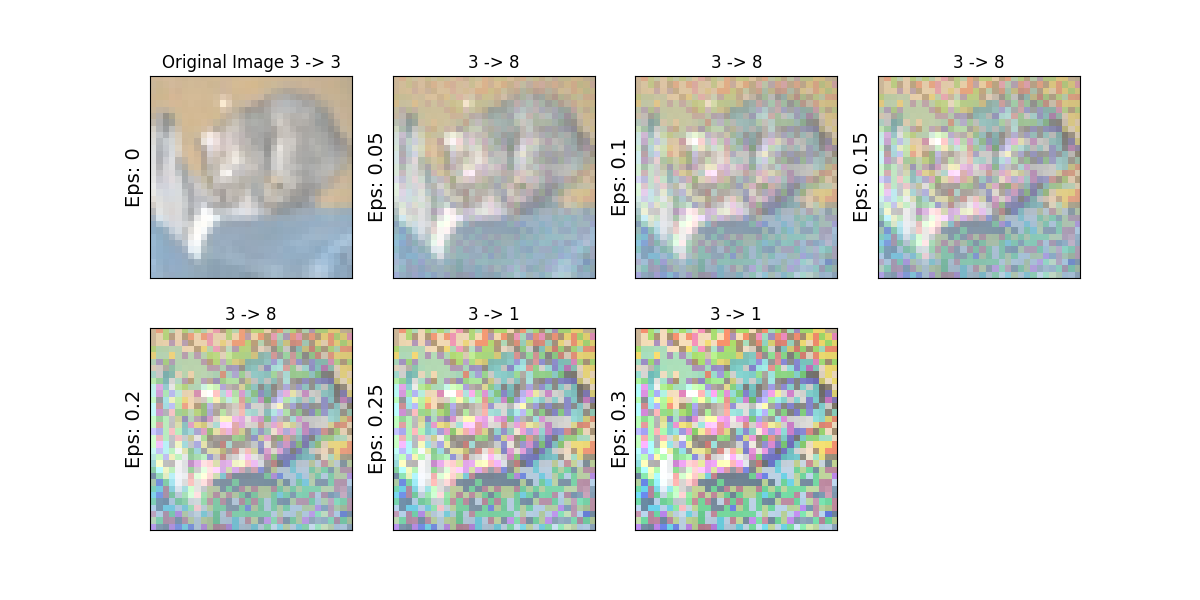
\includegraphics[width=\textwidth]{figures/perturbed_updated.png}
\caption{The first modified image for different values of epsilon.}
\label{fig:perturbed}
\end{figure}




\newpage
\section*{Additional Materials}
\subsection*{TensorBoard}

TensorBoard is a visualization toolkit for neural networks. 
It was originally built for Tensorflow, but also can be used with PyTorch.
The main features of TensorBoard include model visualization, dimenionality reduction, tracking and visualizing metrics, and displaying data.

To create a tensorboard, run the following code:
% imports???
\begin{lstlisting}
>>> %load_ext tensorboard
>>> logs_base_dir = "runs"
>>> os.makedirs(logs_base_dir, exist_ok=True)
>>> %tensorboard --logdir {logs_base_dir}
\end{lstlisting}
The TensorBoard homepage will show up inline:
\begin{figure}[H] % Segmentation example.
    \centering
    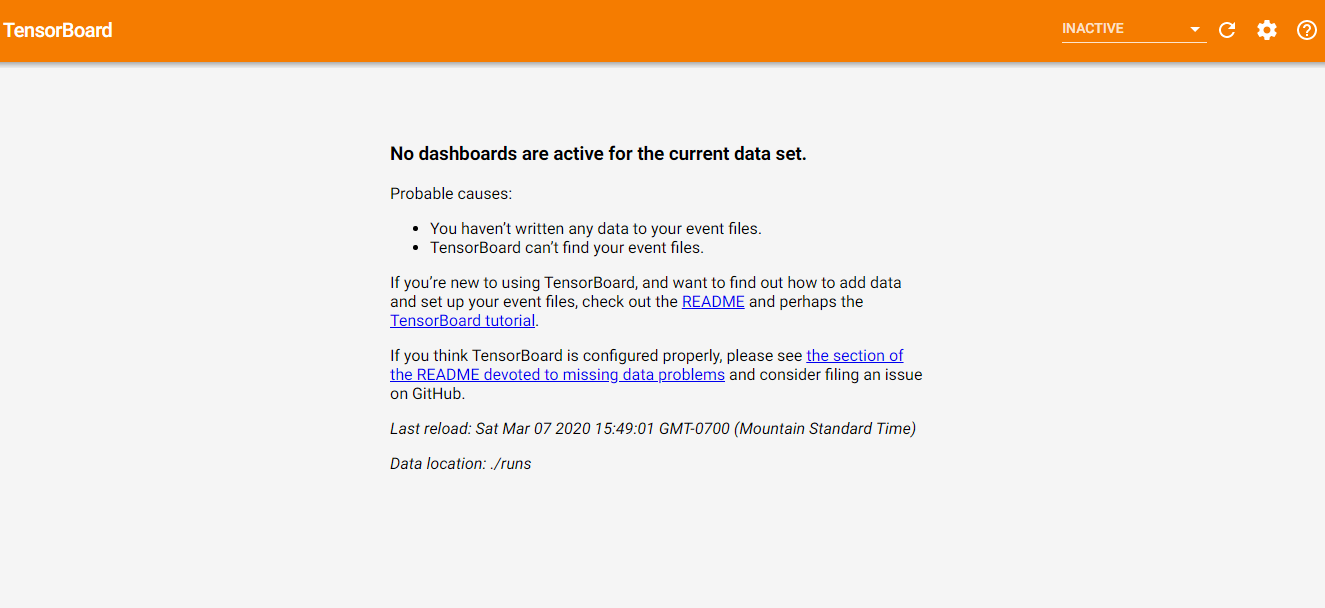
\includegraphics[width=\textwidth]{figures/tensor_board_home.png}

\caption{The home page of an empty TensorBoard.}
\label{fig:tboard_home}
\end{figure}

We write to TensorBoard using \li{SummaryWriter}.
It writes to files in the \li{logs_base_dir} that are used by TensorBoard to display information.
You can view the \li{logs_base_dir} directory by selecting the file icon on the far left of the page.
For example, we can create an interactive graph of our model.

\begin{lstlisting}
>>> tb = SummaryWriter()
>>> tb.add_images("Image", images)
>>> tb.add_graph(model, images)
>>> tb.close()
\end{lstlisting}

This updates our TensorBoard with a \li{GRAPHS} tab, which describes the model.
If it doesn't show up automatically, press the refresh button in the top right corner of the TensorBoard.
You can explore the model by clicking on the components.
\begin{figure}[H] % TensorBoard Graph example.
    \centering
    \begin{subfigure}{.66\textwidth}
        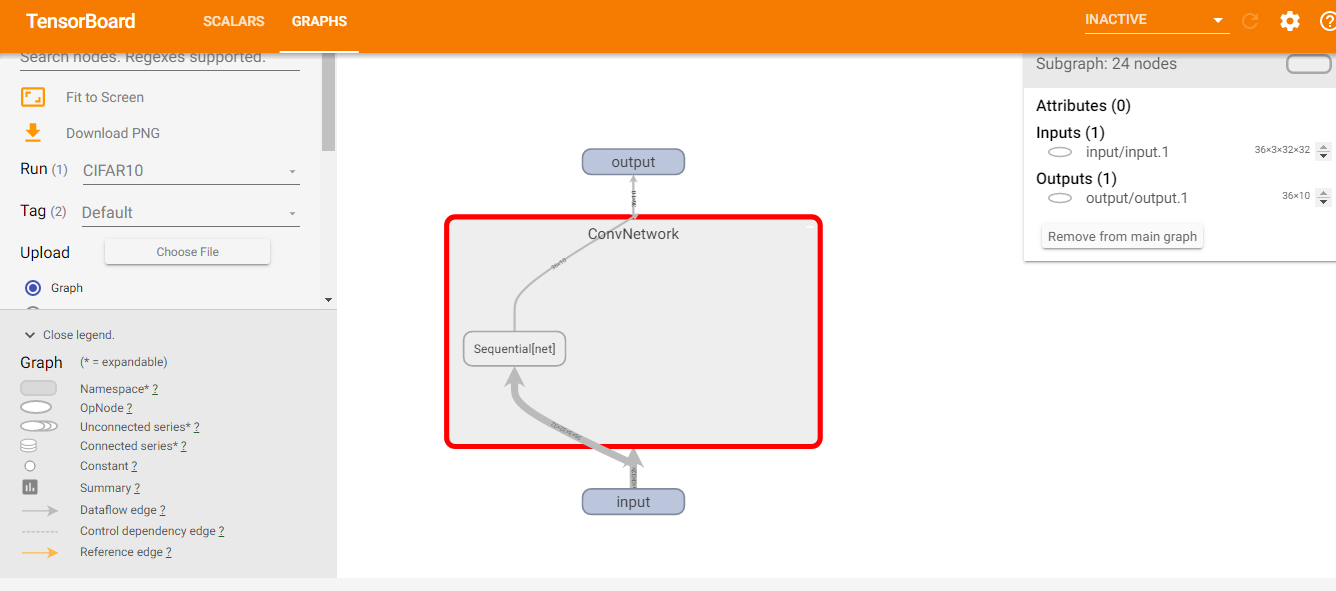
\includegraphics[width=\textwidth]{figures/net1.png}
    \end{subfigure}
    %
    \begin{subfigure}{.66\textwidth}
        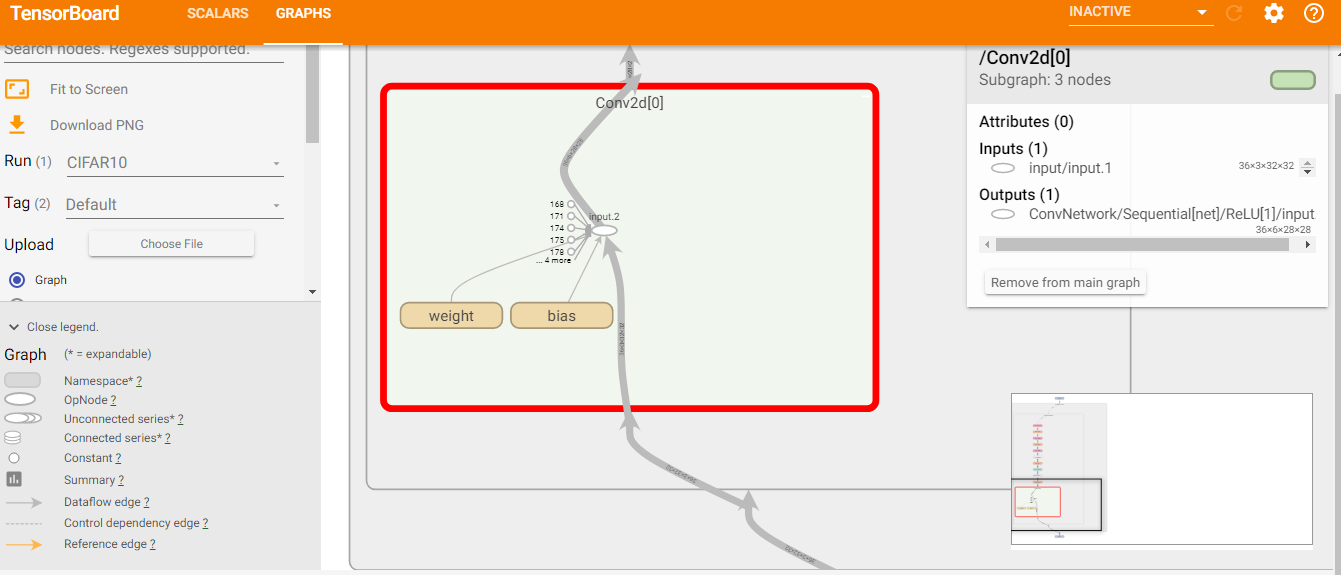
\includegraphics[width=\textwidth]{figures/net2.png}
    \end{subfigure}

\caption{Examples of TensorBoard Graph Tab.}
\label{fig:graphs}
\end{figure}

The following items can be added to TensorBoard, with more information at \url{https://pytorch.org/docs/stable/tensorboard.html}.

\begin{itemize}
\item \li{add_scalar/s}
\item \li{add_image/s}
\item \li{add_figure}
\item \li{add_text}
\item \li{add_graph}
\item \li{add_hparams}

\end{itemize}

To save the training loss, write a function that returns a matplotlib figure of the training loss plot.
Then use \li{tb.add_figure(figure_name, plot_loss())}.

\begin{lstlisting}
writer.add_figure('Training Loss',plot_loss())
\end{lstlisting}

\begin{problem}

Create a TensorBoard for this project that includes the network, a plot of iterations versus training loss and a plot of iterations versus test accuracy from the training done in Problem \ref{prob:train}.

\end{problem}



\begin{comment}
\begin{problem}
Optional Tensorboard Problem


Write a function that randomly chooses four images from the training set, (this can be done through the DataLoader), predicts the labels, and returns a matplotlib figure with the images, the labels with the model's top prediction, its probability, and the actual label.
Remember to unnormalize the images using 

\begin{lstlisting}
>>> img = images[idx]/ 2 + 0.5  }
\end{lstlisting}
Save the figure to tensorboard using \li{add_figure}.


Display a screenshot inline of the image in tensorboard using 
\begin{lstlisting}
>>> from IPython.display import Image
>>> Image('tensorflow.png')
\end{lstlisting}

The Tensorboard Image tab should look like Figure \ref{fig:images}
\end{problem}


\begin{figure}[H]
\centering
\includegraphics[width=\textwidth]{figures/images.png}

\caption{Example of TensorBoard Image Tab displaying four random images with their predicted labels and actual labels.}
\label{fig:images}
\end{figure}
\end{comment}